\documentclass[a4paper,12pt]{article}
\usepackage[utf8]{inputenc}
\usepackage[T2A]{fontenc}
\usepackage[russian]{babel}
\usepackage{amsmath,amssymb}
\usepackage{hyperref}
\usepackage{geometry}
\usepackage{graphicx}
\usepackage{float}
\usepackage{titlesec}
\usepackage{url}
\usepackage{listings}
\hypersetup{hidelinks}
\geometry{top=2cm, bottom=2cm, left=2cm, right=2cm}
\setlength{\parindent}{1.25cm}
\setlength{\parskip}{0pt}

% Формат заголовков
\titleformat{\section}{\normalfont\Large\bfseries\centering}{\thesection.}{1em}{}
\titleformat{\subsection}{\normalfont\large\bfseries}{\thesubsection.}{1em}{}

\hypersetup{hidelinks}

\begin{document}

% Титульный лист
\begin{titlepage}
\begin{center}
\textbf{МИНИСТЕРСТВО НАУКИ И ВЫСШЕГО ОБРАЗОВАНИЯ РОССИЙСКОЙ ФЕДЕРАЦИИ} \\[0.5cm]
\textbf{Федеральное государственное автономное образовательное учреждение высшего образования} \\[0.5cm]
\textbf{«Национальный исследовательский Нижегородский государственный университет им. Н.И. Лобачевского»} \\[0.5cm]
Институт информационных технологий, математики и механики \\
\vfill
{\Large
\textbf{Отчёт по лабораторной работе на тему:} \\[0.5cm]
\textbf{Построение выпуклой оболочки – проход Джарвиса.} \\
}
\vfill
\begin{flushright}
Выполнила: студент группы 3822Б1ФИ1 \\
Направление 02.03.02 \\
«Фундаментальная информатика и информационные технологии» \\
Бесхмельнова Ксения \\
\vspace{1cm}
Преподаватель: \\
Сысоев Александр Владимирович, доцент, кандидат технических наук \\
\end{flushright}
\vfill
Нижний Новгород \\
2024
\end{center}
\end{titlepage}

% Оглавление
\tableofcontents
\newpage

% Введение
\section{Введение}
Задача построения выпуклой оболочки точек имеет фундаментальное значение как в теоретической, так и в прикладной геометрии. Она находит широкое применение в таких областях, как компьютерная графика, обработка изображений, моделирование физических процессов и анализ больших данных. Выпуклая оболочка набора точек представляет собой минимальный выпуклый многоугольник, содержащий все точки из исходного множества.

Однако с увеличением объема входных данных вычислительная сложность задач построения выпуклой оболочки существенно возрастает. Для повышения производительности и сокращения времени вычислений применяются методы параллельного и распределенного программирования. Одним из таких подходов является использование библиотеки MPI (Message Passing Interface), которая предоставляет возможности эффективного взаимодействия между процессами в распределенной системе.

Для построения выпуклой оболочки используются разные алгоритмы. В данной работе реализуется алгоритм Джарвиса.

\newpage

% Постановка задачи
\section{Постановка задачи}
Дана конечная совокупность $S$ точек на плоскости: $S = \{(x_1, y_1), (x_2, y_2), \dots, (x_n, y_n)\}$, где каждая точка задается своими координатами $x$ и $y$. Необходимо определить множество $H \subseteq S$, такое что:
\begin{enumerate}
    \item $H$ является минимальным выпуклым многоугольником, содержащим все точки множества $S$.
    \item Любая точка множества $S$ находится либо на границе $H$, либо внутри него.
\end{enumerate}

Иными словами, требуется построить выпуклую оболочку множества точек $S$, которая является выпуклым замкнутым контуром, охватывающим все точки.

\textbf{Входные данные:}
\begin{itemize}
    \item Множество $S$ из $n$ точек на плоскости, где каждая точка задается координатами $(x_i, y_i)$, $i = 1, \ldots, n$.
\end{itemize}

\textbf{Выходные данные:}
\begin{itemize}
    \item Последовательность точек $H = \{ h_1, h_2, \ldots, h_k \}$, где $h_i \in S$, представляющая вершины выпуклого многоугольника в порядке обхода против часовой стрелки.
\end{itemize}

\newpage

% Описание алгоритма
\section{Описание алгоритма}
Алгоритм Джарвиса (Jarvis March) предназначен для построения выпуклой оболочки множества точек на плоскости. Его ключевая идея заключается в пошаговом добавлении точек, которые формируют контур минимального выпуклого многоугольника.

\textbf{Шаги алгоритма:}
\begin{enumerate}
    \item \textbf{Выбор начальной точки:} 
	\begin{itemize}
		\item Находится точка с минимальной координатой $y$ (или с минимальной $x$, если несколько точек имеют одинаковую $y$) — это гарантирует, что алгоритм начнется с угловой точки оболочки.
	\end{itemize}
    \item \textbf{Поиск следующей точки:} 
	\begin{itemize}
		\item Для текущей точки определяется следующая точка, которая образует наибольший левый угол относительно всех других точек.
		\item Угол определяется по знаку и величине векторного произведения.
	\end{itemize}
    \item \textbf{Обход множества точек:}
	\begin{itemize}
		\item Выбранная точка добавляется в оболочку.
		\item Процесс повторяется до тех пор, пока алгоритм не вернется к начальной точке.
	\end{itemize}
    \item \textbf{Вывод результата:}
	\begin{itemize}
		\item Множество точек, образующих контур, выводится в порядке обхода.
	\end{itemize}
\end{enumerate}

\textbf{Сложность алгоритма:}

Алгоритм имеет временную сложность $O(nh)$, где $n$ — число точек, а $h$ — число точек на выпуклой оболочке. Это делает его более эффективным для малых $h$, но менее подходящим для больших оболочек в больших массивах данных.

\newpage

% Описание схемы распараллеливания
\section{Описание схемы распараллеливания}
Алгоритм Джарвиса, будучи последовательным по своей природе, может быть адаптирован для выполнения в параллельной среде с использованием подходов к разделению данных и распределению вычислений между процессами. Основные шаги распараллеливания включают:
\begin{enumerate}
    \item \textbf{Разделение данных:}

Область точек разбивается на подмножества, которые распределяются между процессами. Каждое подмножество обрабатывается независимо для поиска локальной выпуклой оболочки. Для этого:
	\begin{itemize}
		\item Главный процесс определяет общее количество точек и передает их каждому процессу.
		\item Используется функция определения количества точек, обрабатываемых каждым процессом, в зависимости от его ранга и количества процессов.
	\end{itemize}
    \item \textbf{Параллельное вычисление локальных выпуклых оболочек:}

Каждый процесс вычисляет свою локальную выпуклую оболочку для переданных точек, применяя алгоритм Джарвиса. Для этого:
	\begin{itemize}
		\item Каждое подмножество обрабатывается как самостоятельный набор точек.
		\item Результатом работы каждого процесса является набор точек, образующих локальную выпуклую оболочку.
	\end{itemize}
    \item \textbf{Сбор результатов:}

После завершения локальных вычислений результаты передаются в главный процесс:
\begin{itemize}
		\item Главный процесс собирает локальные выпуклые оболочки.
		\item Эти оболочки объединяются для формирования общего множества точек.
	\end{itemize}
    \item \textbf{Формирование глобальной выпуклой оболочки:}

На последнем этапе главный процесс выполняет последовательный алгоритм Джарвиса на объединенном множестве точек локальных оболочек. Это позволяет устранить промежуточные точки и сформировать окончательную выпуклую оболочку.
\end{enumerate}

\textbf{Оптимизация коммуникаций:}
\begin{itemize}
    \item Значительное ускорение для задач с большим числом точек.
    \item Возможность масштабирования на большое количество процессов.
\end{itemize}

\textbf{Преимущества схемы:}
\begin{itemize}
    \item Значительное ускорение для задач с большим числом точек.
    \item Возможность масштабирования на большое количество процессов.
\end{itemize}

\textbf{Ограничения:}
\begin{itemize}
    \item Накладные расходы на коммуникации между процессами.
    \item Сложность балансировки нагрузки при распределении точек.
\end{itemize}

Эта схема распараллеливания позволяет эффективно использовать ресурсы многопроцессорной среды для задачи построения выпуклой оболочки.

\newpage

% Описание программной реализации MPI-версии алгоритма Джарвиса
\section{Описание программной реализации MPI-версии алгоритма Джарвиса}
Обработка данных:
\begin{itemize}
    \item Входные данные (координаты точек) передаются через массивы inputs.
    \item После завершения вычислений результаты (размер оболочки и координаты её вершин) записываются в массивы outputs.
\end{itemize}

\textbf{Основные этапы выполнения:}
\begin{enumerate}
    \item \textbf{Инициализация (pre\_processing):} на этом этапе точки распределяются между процессами.
    \item \textbf{Валидация (validation):} проверка корректности входных данных (достаточное количество точек, правильный формат).
    \item \textbf{Выполнение (run):} выполняются локальные вычисления и сборка результатов.
    \item \textbf{Постобработка (post\_processing):} результаты вычислений копируются в выходные массивы для дальнейшего использования.
\end{enumerate}

\textbf{Основные функции:}
\begin{itemize}
    \item \textbf{Функция localNumPoints:} определяет, сколько точек обрабатывается каждым процессом в зависимости от их общего количества, количества процессов и текущего ранга.
    \item \textbf{Функция crossProduct:} вычисляет векторное произведение трёх точек.
    \item \textbf{Функция isLeftAngle:} используя векторное произведение, проверяет, образуют ли точки левый поворот.
    \item \textbf{Функция jarvisMarch:} основная последовательная реализация алгоритма Джарвиса для вычисления выпуклой оболочки.
\end{itemize}

\textbf{Особенности параллельной реализации:}
\begin{itemize}
    \item Используются механизмы передачи сообщений (send/recv) для обмена данными между процессами.
    \item Широковещательная передача (broadcast) используется для синхронизации количества точек.
    \item Все вычисления локализованы, а объединение результатов выполняется только на главном процессе.
    \item Программа реализована с использованием шаблонов C++ для работы с различными типами данных.
\end{itemize}

\newpage

% Результаты экспериментов
\section{Результаты экспериментов}
\textbf{Проведенные эксперименты:}
Для оценки производительности и корректности работы параллельной версии алгоритма выпуклой оболочки были проведены следующие эксперименты:

\begin{enumerate}
\item\textbf{Функциональные тесты:}
\begin{itemize}
    \item Проверка корректности работы алгоритма на наборе тестовых данных. 
    \item Использовались различные конфигурации входных данных, например, где выпуклая оболочка представляла собой треугольник или квадрат, многоугольники в разных тестах содержали внутри себя набор случайных точек. Кроме того, были проведены тесты для точек разных типов данных (в частности int и double).

\end{itemize}

\item\textbf{Тесты производительности:}
\begin{itemize}
    \item Оценка времени выполнения алгоритма в параллельном и последовательном режимах.
    \item Сравнение результатов и времени работы для определения преимуществ параллельной версии.
    \item Для измерения времени работы использовались атрибуты производительности ppc::core::PerfAttr с использованием высокоточных таймеров из библиотеки Boost.
    \item Каждое исполнение тестировалось в течение 10 итераций, чтобы получить статистически значимые данные о производительности.
\end{itemize}
\end{enumerate}

\textbf{Подтверждение корректности:}
корректность работы алгоритма подтверждена следующими шагами:
\begin{enumerate}
    \item Сравнение результата работы алгоритма с заранее известными ожидаемыми результатами для тестового набора.
    \item Сравнение выходных данных параллельного и последовательного исполнения (во всех случаях результаты совпали).
    \item Использование инструментов тестирования Google Test для автоматической проверки утверждений (методы \texttt{EXPECT\_EQ} и \texttt{ASSERT\_EQ}).
    \item Многократное повторение экспериментов для устранения случайных ошибок.
\end{enumerate}

Алгоритм успешно справляется с различными наборами точек и правильно формирует границу выпуклой оболочки.


\textbf{Результаты экспериментов:}
результаты тестирования демонстрируют производительность параллельной реализации алгоритма:

\begin{itemize}
    \item \textbf{Для набора данных из 1000 точек:}
    \begin{itemize}
        \item Последовательная версия выполнялась за 0.35–0.40 секунд.
        \item Параллельная версия выполнялась за 0.09–0.12 секунд.
    \end{itemize}
    \begin{figure}[H]
    	\centering
    	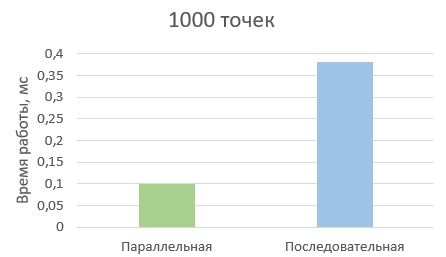
\includegraphics[width=0.8\textwidth]{images/compare_1000.jpg} 
    	\caption{Сравнение времени выполнения для 1000 точек.}
    	\label{fig:compare_1000}
    \end{figure}	
    Таким образом, для 1000 точек параллельная версия алгоритма работает в 3–4 раза быстрее, в зависимости от числа процессов.
    
    \item \textbf{Для набора данных из 10 000 точек:}
    \begin{itemize}
        \item Последовательная версия демонстрирует линейный рост времени выполнения, достигнув 4.5–5 секунд.
        \item Параллельная версия сохраняет свою эффективность, выполняясь примерно за 1.2–1.5 секунды.
    \end{itemize}
    \begin{figure}[H]
    	\centering
    	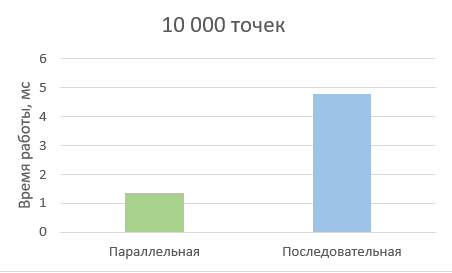
\includegraphics[width=0.8\textwidth]{images/compare_10000.jpg} 
    	\caption{Сравнение времени выполнения для 10000 точек.}
    	\label{fig:compare_10000}
    \end{figure}	
    То есть на 10 000 точек параллельная версия показывает преимущество более чем в 3.5 раза.

    \item \textbf{Для набора данных из 1 000 000 точек:}
    \begin{itemize}
        \item Этот эксперимент проводился лишь для параллельной реализации. Тесты были проведены на количестве процессов от 1 до 8.
    \end{itemize}
    \begin{figure}[H]
    	\centering
    	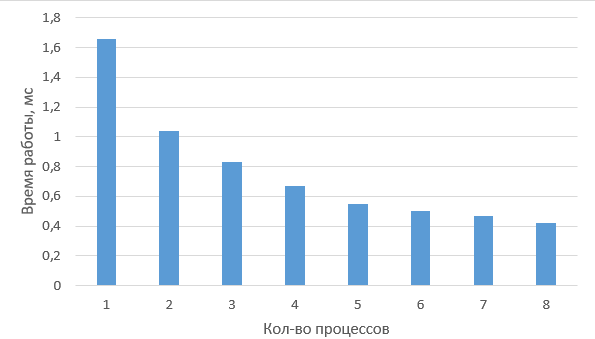
\includegraphics[width=0.8\textwidth]{images/perf_tests_1mln.jpg} 
    	\caption{График зависимости времени работы от количества процессов (1 000 000 точек).}
    	\label{fig:perf_tests_1mln}
    \end{figure}
	Из графика видно, что с увеличением числа процессов время работы алгоритма сокращается. В частности на 8 процессах оболочка строится в 4 раза быстрее, чем на 1 процессе (то есть в 4 раза быстрее последовательной версии).
\end{itemize}

Таким образом, алгоритм выпуклой оболочки на основе метода Джарвиса в параллельной реализации показал себя эффективным и корректным решением для задач вычислительной геометрии.

\newpage

% Выводы из результатов
\section{Выводы из результатов}
На основании проведённых экспериментов и анализа работы алгоритма можно сделать следующие выводы:

\begin{enumerate}
    \item \textbf{Эффективность параллельной реализации:}
	\begin{itemize}
		 \item Параллельная версия алгоритма демонстрирует значительное ускорение по сравнению с последовательной:
		\begin{itemize}
		        \item Ускорение в 3–4 раза для типичных наборов данных из 1000 точек.
		        \item Преимущество параллельной версии увеличивается с ростом объёма данных, особенно для больших наборов (10 000 точек и более).
	    	\end{itemize}
		\item Такая производительность достигается благодаря распределению вычислений между процессами в среде MPI, что снижает общее время выполнения задачи.
	\end{itemize}
    \item \textbf{Масштабируемость:}
	\begin{itemize}
	        \item Параллельная версия хорошо масштабируется при увеличении числа точек. Это делает алгоритм подходящим для обработки больших объемов данных в условиях ограниченного времени.
	        \item Использование MPI позволяет эффективно распределить вычислительные ресурсы, минимизируя накладные расходы на коммуникацию.
	\end{itemize}
    \item \textbf{Корректность:}
	\begin{itemize}
		\item Алгоритм корректно работает как в последовательной, так и в параллельной реализации. Во всех тестах результаты совпадали с ожидаемыми.
		\item Проверка функциональных тестов с заранее известными результатами подтвердила точность работы алгоритма.
		\item Использование автоматизированного тестирования (Google Test) для утверждений о равенстве результатов укрепило уверенность в корректности.
	\end{itemize}
    \item \textbf{Практическое применение:}
	\begin{itemize}
	        \item Параллельная версия алгоритма особенно эффективна для задач, связанных с обработкой больших данных, таких как:
			\begin{itemize}
				\item Компьютерное зрение.
				\item Географические информационные системы (ГИС).
				\item Анализ данных в распределённых вычислительных системах.
			\end{itemize}
	        \item Алгоритм подходит для многопроцессорных сред и кластеров, где MPI может использоваться для достижения высокой производительности.
	    \end{itemize}
\end{enumerate}

\textbf{Общий вывод:}
Метод Джарвиса в параллельной реализации показал высокую производительность, масштабируемость и точность. Результаты экспериментов подтверждают, что использование параллельных вычислений существенно ускоряет обработку данных, обеспечивая значительные преимущества по времени выполнения без потери качества вычислений.

\newpage

% Заключение
\section{Заключение}
В ходе работы была выполнена реализация и анализ последовательной и параллельной версий алгоритма построения выпуклой оболочки методом Джарвиса. Основное внимание уделено сравнению производительности обеих реализаций и анализу их корректности. Эксперименты показали, что использование параллельного подхода на основе MPI позволяет существенно ускорить выполнение алгоритма, особенно при работе с большими наборами данных. Это делает предложенный подход перспективным для использования в задачах анализа больших геометрических данных и встраивания в высокопроизводительные вычислительные системы.

Результаты экспериментов подтверждают, что предложенный алгоритм может быть успешно применён для решения реальных задач, связанных с анализом данных в многопроцессорных системах.

\newpage

% Список литературы
\section{Список литературы}
\begin{enumerate}
    \item Boost MPI Library Documentation: \url{https://www.boost.org/doc/libs/release/libs/mpi/}
    \item Chan T.M. Optimal Output-Sensitive Convex Hull Algorithms in Two and Three Dimensions. Discrete \& Computational Geometry, 1996.
    \item Convex hull Algorithm – Graham Scan and Jarvis March tutorial: \url{https://www.youtube.com/watch?v=B2AJoQSZf4M}
    \item Gropp W., Lusk E., Skjellum A. Using MPI: Portable Parallel Programming with the Message Passing Interface. MIT Press, 1994.
    \item Дж. Джарвис. Метод обхода по часовой стрелке для построения выпуклой оболочки. Algorithmica, 1973.
    \item GTest Documentation: \url{https://google.github.io/googletest/}
\end{enumerate}

\newpage

% Приложения
\section{Приложение 1 \texttt{mpi/ beskhmelnova\_k\_jarvis\_march/include/jarvis\_march.hpp}}
{\footnotesize
\begin{lstlisting}
#pragma once

#include <gtest/gtest.h>

#include <boost/mpi.hpp>
#include <boost/mpi/collectives.hpp>
#include <boost/mpi/communicator.hpp>
#include <boost/mpi/environment.hpp>
#include <vector>

#include "core/task/include/task.hpp"

namespace beskhmelnova_k_jarvis_march_mpi {

template <typename DataType>
DataType crossProduct(const std::vector<DataType>& p1, const std::vector<DataType>& p2,
                      const std::vector<DataType>& p3);

template <typename DataType>
bool isLeftAngle(const std::vector<DataType>& p1, const std::vector<DataType>& p2, 
		  const std::vector<DataType>& p3);

template <typename DataType>
void jarvisMarch(int& num_points, std::vector<std::vector<DataType>>& input, 
		std::vector<DataType>& res_x, std::vector<DataType>& res_y);

int localNumPoints(int num_points, int world_size, int rank);

template <typename DataType>
class TestMPITaskSequential : public ppc::core::Task {
 public:
  explicit TestMPITaskSequential(std::shared_ptr<ppc::core::TaskData> taskData_) : 
		Task(std::move(taskData_)) {}

  bool pre_processing() override;
  bool validation() override;
  bool run() override;
  bool post_processing() override;

 private:
  int num_points{};
  std::vector<std::vector<DataType>> input;
  std::vector<DataType> res_x;
  std::vector<DataType> res_y;
};

template <typename DataType>
class TestMPITaskParallel : public ppc::core::Task {
 public:
  explicit TestMPITaskParallel(std::shared_ptr<ppc::core::TaskData> taskData_) : 
		Task(std::move(taskData_)) {}

  bool pre_processing() override;
  bool validation() override;
  bool run() override;
  bool post_processing() override;

 private:
  boost::mpi::communicator world;

  int num_points{};
  std::vector<DataType> input_x;
  std::vector<DataType> input_y;
  std::vector<DataType> res_x;
  std::vector<DataType> res_y;

  int local_num_points{};
  std::vector<DataType> local_input_x;
  std::vector<DataType> local_input_y;
  std::vector<std::vector<DataType>> local_input;
};
}  // namespace beskhmelnova_k_jarvis_march_mpi
\end{lstlisting}
}	

\newpage

\section{Приложение 2 \texttt{mpi/ beskhmelnova\_k\_jarvis\_march/src/jarvis\_march.cpp}}
{\footnotesize
\begin{lstlisting}
#include "mpi/beskhmelnova_k_jarvis_march/include/jarvis_march.hpp"

#include <random>

using namespace std::chrono_literals;

int beskhmelnova_k_jarvis_march_mpi::localNumPoints(int num_points, int world_size, 
		int rank) {
  if (num_points / world_size < 3) {
    if (num_points / 3 <= rank) return 0;
    world_size = num_points / 3;
  }
  if (num_points % world_size <= rank) return num_points / world_size;
  return num_points / world_size + 1;
}

template <typename DataType>
DataType beskhmelnova_k_jarvis_march_mpi::crossProduct(const std::vector<DataType>& p1, 
		const std::vector<DataType>& p2, const std::vector<DataType>& p3) {
  return ((p2[1] - p1[1]) * (p3[2] - p1[2]) - (p3[1] - p1[1]) * (p2[2] - p1[2]));
}

template <typename DataType>
bool beskhmelnova_k_jarvis_march_mpi::isLeftAngle(const std::vector<DataType>& p1, 
		const std::vector<DataType>& p2, const std::vector<DataType>& p3) {
  return cross_product(p1, p2, p3) > 0;
}

template <typename DataType>
void beskhmelnova_k_jarvis_march_mpi::jarvisMarch(int& num_points, 
		std::vector<std::vector<DataType>>& input, std::vector<DataType>& res_x, 
		std::vector<DataType>& res_y) {
  int leftmost_index = 0;
  for (int i = 1; i < num_points; i++)
    if (input[i][1] < input[leftmost_index][1] ||
        (input[i][1] == input[leftmost_index][1] && 
			input[i][2] < input[leftmost_index][2]))
      leftmost_index = i;
  std::swap(input[0], input[leftmost_index]);
  std::vector<std::vector<DataType>> hull;
  int current = 0;
  do {
    hull.push_back(input[current]);
    int next = (current + 1) % num_points;
    for (int i = 0; i < num_points; ++i) {
      auto cross_product =
          beskhmelnova_k_jarvis_march_mpi::crossProduct<DataType>(input[current], 
								input[next], input[i]);
      if (cross_product < 0 || (cross_product == 0 &&
           std::hypot(input[i][1] - input[current][1], input[i][2] - input[current][2]) >
           std::hypot(input[next][1] - input[current][1], 
		input[next][2] - input[current][2])))
        next = i;
    }
    current = next;
  } while (current != 0);
  num_points = static_cast<int>(hull.size());
  res_x.resize(num_points);
  res_y.resize(num_points);
  for (int i = 0; i < num_points; ++i) {
    res_x[i] = hull[i][1];
    res_y[i] = hull[i][2];
  }
  input = hull;
}

template <typename DataType>
bool beskhmelnova_k_jarvis_march_mpi::TestMPITaskSequential<DataType>::pre_processing() {
  internal_order_test();
  num_points = (int)taskData->inputs_count[0];
  input = std::vector<std::vector<DataType>>(num_points, std::vector<DataType>(3, 0));
  auto* ptr_x = reinterpret_cast<DataType*>(taskData->inputs[0]);
  auto* ptr_y = reinterpret_cast<DataType*>(taskData->inputs[1]);
  for (int i = 0; i < num_points; i++) {
    input[i][1] = ptr_x[i];
    input[i][2] = ptr_y[i];
  }
  return true;
}

template <typename DataType>
bool beskhmelnova_k_jarvis_march_mpi::TestMPITaskSequential<DataType>::validation() {
  internal_order_test();
  return taskData->inputs_count[0] >= 3 && taskData->outputs_count.size() == 3;
}

template <typename DataType>
bool beskhmelnova_k_jarvis_march_mpi::TestMPITaskSequential<DataType>::run() {
  internal_order_test();
  jarvisMarch(num_points, input, res_x, res_y);
  return true;
}

template <typename DataType>
bool beskhmelnova_k_jarvis_march_mpi::TestMPITaskSequential<DataType>::post_processing() {
  internal_order_test();
  reinterpret_cast<int*>(taskData->outputs[0])[0] = num_points;
  for (int i = 0; i < num_points; i++) {
    reinterpret_cast<DataType*>(taskData->outputs[1])[i] = input[i][1];
    reinterpret_cast<DataType*>(taskData->outputs[2])[i] = input[i][2];
  }
  return true;
}

template <typename DataType>
bool beskhmelnova_k_jarvis_march_mpi::TestMPITaskParallel<DataType>::pre_processing() {
  internal_order_test();
  if (world.rank() == 0) {
    num_points = (int)taskData->inputs_count[0];
    input_x = std::vector<DataType>(num_points);
    input_y = std::vector<DataType>(num_points);
    auto* ptr_x = reinterpret_cast<DataType*>(taskData->inputs[0]);
    auto* ptr_y = reinterpret_cast<DataType*>(taskData->inputs[1]);
    for (int i = 0; i < num_points; i++) {
      input_x[i] = ptr_x[i];
      input_y[i] = ptr_y[i];
    }
  }
  return true;
}

template <typename DataType>
bool beskhmelnova_k_jarvis_march_mpi::TestMPITaskParallel<DataType>::validation() {
  internal_order_test();
  if (world.rank() == 0) return taskData->inputs_count[0] >= 3 && 
		taskData->outputs_count.size() == 3;
  return true;
}

template <typename DataType>
bool beskhmelnova_k_jarvis_march_mpi::TestMPITaskParallel<DataType>::run() {
  internal_order_test();
  broadcast(world, num_points, 0);
  if (world.rank() == 0) {
    local_num_points = localNumPoints(num_points, world.size(), world.rank());
    local_input_x = std::vector<DataType>(input_x.begin(), 
			input_x.begin() + local_num_points);
    local_input_y = std::vector<DataType>(input_y.begin(), 
			input_y.begin() + local_num_points);
    int sum_next_num_points = local_num_points;
    for (int i = 1; i < world.size(); i++) {
      int next_num_points = localNumPoints(num_points, world.size(), i);
      if (next_num_points != 0) {
        world.send(i, 0, input_x.data() + sum_next_num_points, next_num_points);
        world.send(i, 0, input_y.data() + sum_next_num_points, next_num_points);
      }
      sum_next_num_points += next_num_points;
    }
  } else {
    local_num_points = localNumPoints(num_points, world.size(), world.rank());
    if (local_num_points != 0) {
      local_input_x = std::vector<DataType>(local_num_points);
      local_input_y = std::vector<DataType>(local_num_points);
      world.recv(0, 0, local_input_x.data(), local_num_points);
      world.recv(0, 0, local_input_y.data(), local_num_points);
    }
  }

  if (local_num_points != 0) {
    local_input = std::vector<std::vector<DataType>>(local_num_points, 
							std::vector<DataType>(3, 0));
    for (int i = 0; i < local_num_points; i++) {
      local_input[i][1] = local_input_x[i];
      local_input[i][2] = local_input_y[i];
    }
    std::vector<DataType> local_res_x;
    std::vector<DataType> local_res_y;
    jarvisMarch(local_num_points, local_input, local_res_x, local_res_y);
    local_input_x = local_res_x;
    local_input_y = local_res_y;
  }
  if (world.rank() == 0) {
    input_x.assign(local_input_x.begin(), local_input_x.end());
    input_y.assign(local_input_y.begin(), local_input_y.end());
    int sum_next_num_points = local_num_points;
    for (int i = 1; i < world.size(); i++) {
      int next_num_points;
      world.recv(i, 0, &next_num_points, 1);
      if (next_num_points != 0) {
        world.recv(i, 0, input_x.data() + sum_next_num_points, next_num_points);
        world.recv(i, 0, input_y.data() + sum_next_num_points, next_num_points);
      }
      sum_next_num_points += next_num_points;
    }
    local_num_points = sum_next_num_points;
  } else {
    world.send(0, 0, &local_num_points, 1);
    if (local_num_points != 0) {
      world.send(0, 0, local_input_x.data(), local_num_points);
      world.send(0, 0, local_input_y.data(), local_num_points);
    }
  }
  if (world.rank() == 0) {
    local_input = std::vector<std::vector<DataType>>(local_num_points, 
							std::vector<DataType>(3, 0));
    for (int i = 0; i < local_num_points; i++) {
      local_input[i][1] = input_x[i];
      local_input[i][2] = input_y[i];
    }
    std::vector<DataType> final_res_x;
    std::vector<DataType> final_res_y;
    jarvisMarch(local_num_points, local_input, final_res_x, final_res_y);
    res_x = final_res_x;
    res_y = final_res_y;
  }
  return true;
}

template <typename DataType>
bool beskhmelnova_k_jarvis_march_mpi::TestMPITaskParallel<DataType>::post_processing() {
  internal_order_test();
  if (world.rank() == 0) {
    reinterpret_cast<int*>(taskData->outputs[0])[0] = static_cast<int>(res_x.size());
    for (size_t i = 0; i < res_x.size(); i++) {
      reinterpret_cast<DataType*>(taskData->outputs[1])[i] = res_x[i];
      reinterpret_cast<DataType*>(taskData->outputs[2])[i] = res_y[i];
    }
  }
  return true;
}

template class beskhmelnova_k_jarvis_march_mpi::TestMPITaskSequential<double>;
template class beskhmelnova_k_jarvis_march_mpi::TestMPITaskParallel<double>;

template class beskhmelnova_k_jarvis_march_mpi::TestMPITaskSequential<int>;
template class beskhmelnova_k_jarvis_march_mpi::TestMPITaskParallel<int>;
\end{lstlisting}
}

\newpage

\section{Приложение 3 \texttt{seq/ beskhmelnova\_k\_jarvis\_march/include/jarvis\_march.hpp}}
{\footnotesize
\begin{lstlisting}
#pragma once

#include <vector>

#include "core/task/include/task.hpp"

namespace beskhmelnova_k_jarvis_march_seq {

template <typename DataType>
DataType crossProduct(const std::vector<DataType>& p1, 
	const std::vector<DataType>& p2, const std::vector<DataType>& p3);

template <typename DataType>
bool isLeftAngle(const std::vector<DataType>& p1, 
	const std::vector<DataType>& p2, const std::vector<DataType>& p3);

template <typename DataType>
void jarvisMarch(int& num_points, std::vector<std::vector<DataType>>& input, 
	std::vector<DataType>& res_x, std::vector<DataType>& res_y);

template <typename DataType>
class TestTaskSequential : public ppc::core::Task {
 public:
  explicit TestTaskSequential(std::shared_ptr<ppc::core::TaskData> taskData_) : 
		Task(std::move(taskData_)) {}
  bool pre_processing() override;
  bool validation() override;
  bool run() override;
  bool post_processing() override;

 private:
  int num_points{};
  std::vector<std::vector<DataType>> input;
  std::vector<DataType> res_x;
  std::vector<DataType> res_y;
};

}  // namespace beskhmelnova_k_jarvis_march_seq
\end{lstlisting}
}
\newpage

\section{Приложение 4 \texttt{seq/ beskhmelnova\_k\_jarvis\_march/src/jarvis\_march.cpp}}
{\footnotesize
\begin{lstlisting}
#include "seq/beskhmelnova_k_jarvis_march/include/jarvis_march.hpp"

#include <random>

using namespace std::chrono_literals;

template <typename DataType>
DataType beskhmelnova_k_jarvis_march_seq::crossProduct(const std::vector<DataType>& p1,
	 const std::vector<DataType>& p2, const std::vector<DataType>& p3) {
  return ((p2[1] - p1[1]) * (p3[2] - p1[2]) - (p3[1] - p1[1]) * (p2[2] - p1[2]));
}

template <typename DataType>
bool beskhmelnova_k_jarvis_march_seq::isLeftAngle(const std::vector<DataType>& p1,
	const std::vector<DataType>& p2, const std::vector<DataType>& p3) {
  return cross_product(p1, p2, p3) > 0;
}

template <typename DataType>
void beskhmelnova_k_jarvis_march_seq::jarvisMarch(int& num_points, 
	std::vector<std::vector<DataType>>& input,
          std::vector<DataType>& res_x, std::vector<DataType>& res_y) {
  int leftmost_index = 0;
  for (int i = 1; i < num_points; i++)
    if (input[i][1] < input[leftmost_index][1] ||
        (input[i][1] == input[leftmost_index][1] &&
		 input[i][2] < input[leftmost_index][2]))
      leftmost_index = i;
  std::swap(input[0], input[leftmost_index]);
  std::vector<std::vector<DataType>> hull;
  int current = 0;
  do {
    hull.push_back(input[current]);
    int next = (current + 1) % num_points;
    for (int i = 0; i < num_points; ++i) {
      auto cross_product =
          beskhmelnova_k_jarvis_march_seq::crossProduct<DataType>(input[current], 
			input[next], input[i]);
      if (cross_product < 0 || (cross_product == 0 &&
          std::hypot(input[i][1] - input[current][1], input[i][2] - input[current][2]) >
          std::hypot(input[next][1] - input[current][1], 
		 input[next][2] - input[current][2])))
        next = i;
    }
    current = next;
  } while (current != 0);
  num_points = static_cast<int>(hull.size());
  res_x.resize(num_points);
  res_y.resize(num_points);
  for (int i = 0; i < num_points; ++i) {
    res_x[i] = hull[i][1];
    res_y[i] = hull[i][2];
  }
  input = hull;
}

template <typename DataType>
bool beskhmelnova_k_jarvis_march_seq::TestTaskSequential<DataType>::pre_processing() {
  internal_order_test();
  num_points = (int)taskData->inputs_count[0];
  input = std::vector<std::vector<DataType>>(num_points, std::vector<DataType>(3, 0));
  auto* ptr_x = reinterpret_cast<DataType*>(taskData->inputs[0]);
  auto* ptr_y = reinterpret_cast<DataType*>(taskData->inputs[1]);
  for (int i = 0; i < num_points; i++) {
    input[i][1] = ptr_x[i];
    input[i][2] = ptr_y[i];
  }
  return true;
}

template <typename DataType>
bool beskhmelnova_k_jarvis_march_seq::TestTaskSequential<DataType>::validation() {
  internal_order_test();
  return taskData->inputs_count[0] >= 3 && taskData->outputs_count.size() == 3;
}

template <typename DataType>
bool beskhmelnova_k_jarvis_march_seq::TestTaskSequential<DataType>::run() {
  internal_order_test();
  jarvisMarch(num_points, input, res_x, res_y);
  return true;
}

template <typename DataType>
bool beskhmelnova_k_jarvis_march_seq::TestTaskSequential<DataType>::post_processing() {
  internal_order_test();
  reinterpret_cast<int*>(taskData->outputs[0])[0] = num_points;
  for (int i = 0; i < num_points; i++) {
    reinterpret_cast<DataType*>(taskData->outputs[1])[i] = input[i][1];
    reinterpret_cast<DataType*>(taskData->outputs[2])[i] = input[i][2];
  }
  return true;
}

template class beskhmelnova_k_jarvis_march_seq::TestTaskSequential<double>;
\end{lstlisting}
}
\end{document}
